\documentclass[9pt]{extarticle}

\usepackage[margin=0.6in]{geometry}
\usepackage{amsmath,amssymb}
\usepackage{booktabs}
\usepackage{enumitem}
\usepackage{tikz}
\usetikzlibrary{arrows.meta,positioning}
\usepackage{microtype}
\usepackage{parskip}
\usepackage{titlesec}
\usepackage[hyphens]{url}
\usepackage[colorlinks=true,linkcolor=black,urlcolor=blue]{hyperref}
\Urlmuskip=0mu plus 1mu\relax

\titleformat{\section}{\normalfont\normalsize\bfseries}{\thesection.}{0.5em}{}
\titlespacing*{\section}{0pt}{0.7em}{0.2em}
\setlength{\parskip}{0.15em}
\setlist[itemize]{leftmargin=1.5em,itemsep=0.15em,topsep=0.2em,parsep=0em}
\pagestyle{empty}

\newcommand{\ck}{\item[$\square$]}


\tikzset{
  blk/.style={draw,rounded corners=2pt,minimum width=20mm,minimum height=6mm,font=\scriptsize,align=center,line width=0.3pt},
  pred/.style={blk,dashed},
  ar/.style={-{Stealth[length=1.4mm]},line width=0.35pt},
  lbl/.style={font=\scriptsize\itshape,align=center},
  hd/.style={font=\small\bfseries}
}
\begin{document}

\begin{center}
{\large \textbf{Does Dynamics Prediction Make Policies Robust to Changed Dynamics?}}\\[0.1em]
{\footnotesize Design rationale and build checklist in one document. Gates marked in bold. v0.2}
\end{center}

\textbf{Part I sets out why the experiment is worth running and what each arm is for. Part II is the ordered build. Read Part I once, work from Part II.}

\begin{center}\rule{0.35\textwidth}{0.4pt}\end{center}
\begin{center}{\small\bfseries PART I. RATIONALE}\end{center}

\section{What is being asked, and why it is open}

The belief in the field is that adding a next-state prediction objective to a policy makes it generalize better, because the policy learns how the world works. Two separate things must be checked, and neither has been.

\textbf{The effect has not been measured on the right axis.} Every published comparison between prediction-trained systems (call them P+) and imitation-only systems (P$-$) changes \emph{appearance} at test time: lighting, backgrounds, distractor objects, camera angle, novel object looks, language phrasing. DAP, LaDi-WM, and the recent world-action-model robustness study all sit here. Separately, a body of work does change physical parameters such as mass, friction and gravity, but every arm in those comparisons is itself prediction-based: CaDM, IIDA, RMA, AnyCar and DALI compare dynamics models against other dynamics models, never against a diffusion or flow policy. The intersection, P+ against P$-$ under a change of physical dynamics, is empty. So the first thing to fix is the framing: this is an open question, not a settled fact to build on.

\textbf{The mechanism has not been tested at all.} Adding a prediction head changes four things at once besides physics. It gives the trunk a second job, which discourages memorisation. It supplies many more supervised numbers per sample, since a state has more dimensions than an action, so the network learns faster from the same data. It adds a smooth, dense loss to a noisy generative one, which stabilises optimisation. And it forces states with similar futures to sit near each other internally, which tidies the representation. Each of these can produce the same improvement with no physics learned. There is published support for the fourth and second in particular: Fang et al.\ show that modest latent representation error acts as implicit regularisation and can improve world model robustness, and BYOL-$\gamma$ found that minimal one-step next-state prediction gives almost no benefit over plain behaviour cloning, with the gains instead coming from temporally extended structure. So the deflationary outcome is not hypothetical. It has already happened once for a closely related objective.

The experiment therefore has two halves: establish whether the effect exists on the dynamics axis, then determine what causes it.

\section{What differs between arms, and why it must}

Let $h$ be the recent history of states and actions, $\phi_\theta$ a shared trunk, and $c$ the hidden physical parameters, drawn per episode and never shown to the network.

\textbf{Base (P$-$)}, a flow policy with an action target only:
\[
\mathcal{L}_{\text{base}} = \mathbb{E}\big\| v_\theta(a^\tau, \tau, \phi(h)) - (a_1 - a_0) \big\|^2 .
\]

\textbf{Treatment (P+)}, the identical network with one extra head:
\[
\mathcal{L}_{\text{treat}} = \mathcal{L}_{\text{base}} + \lambda \cdot \mathbb{E}\big\| g_\theta(\phi(h), a) - x_{t+1} \big\|^2 .
\]

Only the second term differs. Same dataset, same trunk architecture, same parameter budget, same optimiser, same seeds.

\subsection{Why the constraints are constraints}

\textbf{Identical data.} DAP trains its dynamics model on expert plus random exploration data while its policy sees expert data only, so the treatment arm receives roughly twice the data. Any gap could then be data volume rather than the objective. This is the single choice that stops DAP being a clean test of its own claim, and it costs nothing to avoid.

\textbf{Change physics, freeze appearance.} Sweep mass, friction, damping, payload and actuator gain while keeping the visual scene fixed. If appearance and physics move together, the result reproduces the existing literature's confound and adds nothing.

\textbf{Identical controller.} A world model paired with planning searches at inference; a policy simply emits an action. If the prediction arm degrades more slowly while also planning, the cause could be planning rather than knowledge. Both arms reactive, or both planning. Never one of each.

\textbf{Slopes, not points.} The claim is about the \emph{rate} of decay under shift, which a single held-out test point cannot express.

\section{The three arms}

Three arms. Two of them form the controlled contrast that carries the argument; the third is a reference point for what the field actually builds.

\begin{center}
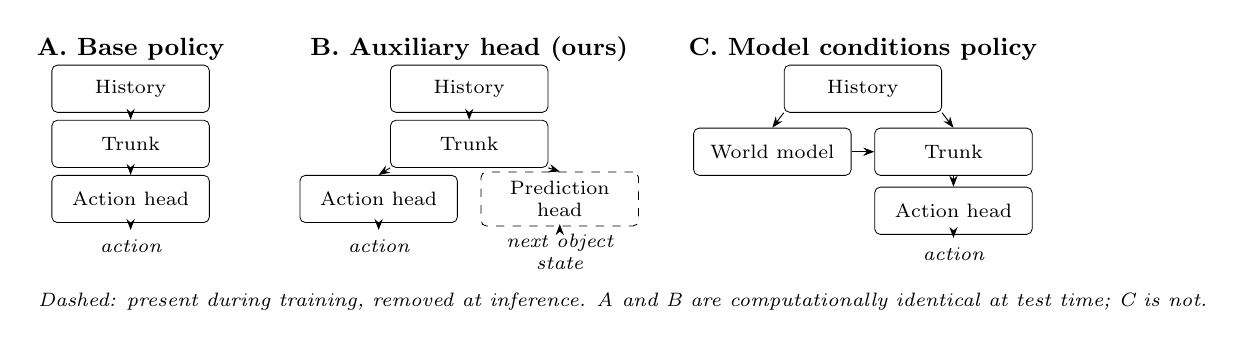
\begin{tikzpicture}[node distance=5mm]

\node[hd] at (0,1.05) {A. Base policy};
\node[blk] (ah) at (0,0.55) {History};
\node[blk] (at) at (0,-0.15) {Trunk};
\node[blk] (aa) at (0,-0.85) {Action head};
\node[lbl] (aact) at (0,-1.45) {action};
\draw[ar] (ah)--(at); \draw[ar] (at)--(aa); \draw[ar] (aa)--(aact);

\node[hd] at (4.3,1.05) {B. Auxiliary head (ours)};
\node[blk] (bh) at (4.3,0.55) {History};
\node[blk] (bt) at (4.3,-0.15) {Trunk};
\node[blk] (ba) at (3.15,-0.85) {Action head};
\node[pred] (bp) at (5.45,-0.85) {Prediction\\head};
\node[lbl] (bact) at (3.15,-1.45) {action};
\node[lbl] (bpr) at (5.45,-1.52) {next object\\state};
\draw[ar] (bh)--(bt); \draw[ar] (bt.south west)--(ba.north); \draw[ar] (bt.south east)--(bp.north);
\draw[ar] (ba)--(bact); \draw[ar] (bp)--(bpr);

\node[hd] at (9.3,1.05) {C. Model conditions policy};
\node[blk] (ch) at (9.3,0.55) {History};
\node[blk] (cw) at (8.15,-0.25) {World model};
\node[blk] (ct) at (10.45,-0.25) {Trunk};
\node[blk] (ca) at (10.45,-1.0) {Action head};
\node[lbl] (cact) at (10.45,-1.55) {action};
\draw[ar] (ch.south west)--(cw.north); \draw[ar] (ch.south east)--(ct.north); \draw[ar] (cw)--(ct);
\draw[ar] (ct)--(ca); \draw[ar] (ca)--(cact);

\node[lbl,anchor=west] at (-1.3,-2.15) {Dashed: present during training, removed at inference. A and B are computationally identical at test time; C is not.};
\end{tikzpicture}
\end{center}

\textbf{Arm A, base.} A flow-matching policy in the Diffusion Policy mould: action chunking over a short horizon, a history encoder over the last $K$ observations, and a velocity-field head trained by the rectified-flow objective. State input at roughly 1 to 10M parameters; the vision variant uses a ResNet-18 or ViT-S encoder into the same trunk at roughly 20 to 50M. Train from scratch. A pretrained checkpoint has seen data the other arm has not, which breaks the single constraint that makes the comparison mean anything.

\textbf{Arm B, treatment.} The identical trunk with a two-layer MLP prediction head attached. The head is the only structural difference and $\lambda$ the only new hyperparameter, and it is discarded after training. This is what makes B the instrument: at deployment A and B are the same network running the same forward pass, so a difference in degradation cannot be attributed to extra computation or extra information at inference. It is also why the shuffled-target control works, since the head, its gradients and its constraint on the trunk can all be preserved while only the content of its target is destroyed.

The prediction target is the \emph{object's} future state, not the robot's. Predicting the arm's next joint configuration is nearly free, since the controller largely determines it, and a policy can do that well while knowing nothing about the object. Target the object pose and velocity, which is where $c$ actually enters.

\textbf{Three target types within arm B, not one.} BYOL-$\gamma$ found that a minimal one-step next-state target confers almost no benefit over plain behaviour cloning, with gains appearing only once the target became temporally extended. If the treatment uses a one-step target alone, a null is already explained by their result. So run: one-step object state; multi-step object state over $H$ of 5 to 10; and latent with stop-gradient, $\|g_\theta(\phi(h),a) - \mathrm{sg}[\phi(x_{t+1})]\|^2$. Target type becomes a reported axis, and the result connects to the self-predictive literature rather than sitting beside it.

\textbf{Arm C, reference.} The same trained prediction module, but kept at inference and feeding its forecast into the action head as conditioning. This is the configuration most published hybrids actually use, LaDi-WM and UVA among them, and omitting it invites the objection that the study examined a simplified setting rather than the methods people build.

C is a reference arm and never enters the mediation tests. The reason is that it changes three things at once relative to A: a second network exists, it runs at deployment, and its output enters the policy's forward pass. If C degrades more slowly than B, that could be better learned representation or simply more computation and more information available at test time, and the comparison cannot separate them. So C contributes one number, its degradation slope, reported alongside A and B with that confound stated.

What C does buy, beyond completeness, is a question practitioners care about and a mechanism check that costs nothing. If B and C degrade at similar rates, the second network and its latency are not earning their place, and training with prediction is sufficient. If C is markedly better, the benefit is inference-time information rather than a better-shaped trunk, and the probes should confirm it: C's trunk ought to carry no more decodable $c$ than B's. Either outcome is informative, and the arm is cheap, since C is arm B's prediction head kept at inference rather than a new training pipeline.

\textbf{Not run: bidirectional coupling.} DAP's configuration, where policy and dynamics model exchange information during action generation, is cited as motivation and not reproduced. Its removal ablation takes out the objective, the second network and the coupling mechanism simultaneously, so it is confounded in every direction and cannot serve as an instrument.

\textbf{Controller.} All three arms emit actions directly. None plans. A planning comparison is a separate experiment with its own controls, since inference-time search is a further source of robustness that cannot be separated from knowledge after the fact.

\section{The task ladder}

Three tasks of increasing difficulty, chosen so that each one raises how much of the outcome is determined by physics the policy could not observe. This gives a \emph{predicted ordering} of effect size, which is a stronger result than one large number on one task.

\begin{tabular}{@{}p{1.1cm} p{5.4cm} p{4.6cm} p{5.1cm}@{}}
\toprule
Task & What the robot does & What is unobservable & Why it is harder \\
\midrule
T1 & Push a cube to a target and stop it there & mass, friction & Heavy cubes overshoot. The policy must anticipate momentum, not react to it \\
T2 & Push a cube so it slides free and comes to rest on the target & mass, friction & The robot loses contact partway. The final position depends entirely on a slide the policy had to predict in advance \\
T3 & T2 plus a target orientation & mass, friction, COM offset & An off-centre mass makes the cube rotate when pushed straight. The offset is invisible from any single frame and can only be inferred from the rotation it causes \\
\bottomrule
\end{tabular}

T2 is the primary task. T1 is the fallback if T2 proves too hard to learn at all, and T3 is the extension if the effect is visible in T2. Add a fourth control task, pick-and-place, where the object is rigid to the gripper once grasped and its properties stop mattering. The effect should be near zero there. An effect that appears equally on the control task is evidence against the dynamics account.

\section{Rationale: measuring the effect}

Let $\delta = \|c_{\text{test}} - \mathbb{E}[c_{\text{train}}]\|$ be shift magnitude and $R(\delta)$ the expected regret at that shift. Measure $R_{\text{base}}(\delta)$ and $R_{\text{treat}}(\delta)$ over a grid of $\delta$, with $n \geq 10$ seeds per point, and fit degradation slopes
\[
s_{\text{base}} = \frac{dR_{\text{base}}}{d\delta}, \qquad s_{\text{treat}} = \frac{dR_{\text{treat}}}{d\delta}.
\]
The hypothesis is $s_{\text{treat}} < s_{\text{base}}$.

\textbf{Decision rule, fixed now.} If the confidence intervals on the two slopes overlap, the claim is falsified and that is the result. Given that nobody has measured $s$ on the dynamics axis at all, a null is publishable rather than a failure. Deciding this in advance is what prevents the outcome being reinterpreted after the fact.

\textbf{Precondition.} Before anything else, verify the base policy can actually fail. Train it alone and test on far-out $c$. If it already succeeds, there is no gap to attribute and every later test returns null for uninteresting reasons. Widen the $c$ range, push the held-out values further, or shorten the history until it visibly degrades. One run, and it decides whether the project has a subject.

\section{Rationale: attributing the effect}

Suppose $s_{\text{treat}} < s_{\text{base}}$. Five candidate causes remain: M1 dynamics knowledge, M2 regularisation, M3 gradient density, M4 optimisation conditioning, M5 representation smoothing. Four tests separate them.

\subsection{Test A: shuffled targets}

Replace the prediction target with a batch permutation $\sigma$:
\[
\mathcal{L}_{\text{shuf}} = \mathcal{L}_{\text{base}} + \lambda \cdot \mathbb{E}\big\| g_\theta(\phi(h), a) - \sigma(x_{t+1}) \big\|^2 .
\]
Loss magnitude, gradient count and the constraint on the trunk are all preserved. Only the physics content of the target is destroyed. If $s_{\text{shuf}} \approx s_{\text{treat}}$, then M1 is out and the benefit came from having a second head at all. If $s_{\text{shuf}} \approx s_{\text{base}}$, then M2, M3 and M4 are out, because those survive shuffling by construction. This is the cheapest test available and the only one that can end the enquiry in a single run, so it goes first.

\subsection{Test B: dose response}

Sweep $\lambda$ over roughly twenty values. At each, measure two quantities: $k(\lambda)$, how well $c$ can be decoded from $\phi$ by a probe, and $s(\lambda)$, the degradation slope. If M1 holds, the two are coupled, and $\mathrm{corr}(k(\lambda), -s(\lambda))$ should be near one across the sweep. If $s$ improves while $k$ stays flat, whatever is helping is not knowledge of $c$. If $s$ saturates while $k$ keeps rising, the additional knowledge past that point is not doing any work, and the sweep localises exactly where the useful part ends. Twenty aligned points is a far stronger inference than two conditions differing, which is why this carries the most information per run.

\subsection{Test C: probe then ablate}

Fit a probe $w$ decoding $c$ from $\phi(h)$, then remove that direction at inference:
\[
\phi'(h) = \phi(h) - \frac{w^\top \phi(h)}{\|w\|^2} w, \qquad \Delta s = s(\phi') - s(\phi).
\]
Control with a random unit direction $u$ of matched magnitude, giving $\Delta s_{\text{rand}}$, and report the difference $\Delta s - \Delta s_{\text{rand}}$ rather than the raw drop, since deleting any direction degrades computation somewhat. M1 predicts $\Delta s \gg \Delta s_{\text{rand}}$. This test also fixes a direction-of-causation problem the probes alone cannot: a better policy visits better states and may therefore produce more decodable activations as a consequence of performing well rather than a cause of it. Ablation runs the arrow the right way.

\subsection{Test D: substitution}

Give the base policy, one at a time, an intervention targeting each alternative:
\[
\mathcal{L}_{\text{base}} + \alpha\|\theta\|^2 \;\;(\text{M2}), \qquad
\mathcal{L}_{\text{base}} + \beta\left\|\partial\phi/\partial x\right\|^2 \;\;(\text{M5}),
\]
plus scaling $|D|$ by the supervision ratio $\dim(x)\cdot H / \dim(a)$ for M3, and an extended schedule with tuned learning rate for M4. If any substitution reaches $s \approx s_{\text{treat}}$, that mechanism is sufficient and M1 is unnecessary.

\textbf{This test is worthless without a preregistered budget.} ``Tune weight decay until the gap closes'' has no stopping rule: failure can always be blamed on insufficient search, and success can always be an unrelated optimum. Fix the number of configurations per arm, equal across arms, and the criterion for closing the gap, $|s_{\text{sub}} - s_{\text{treat}}| < \epsilon$, before running anything.

\subsection{Reading the outcome}

\begin{center}
\footnotesize
\begin{tabular}{@{}p{3.3cm} p{3.3cm} p{2.6cm} p{6.4cm}@{}}
\toprule
Test A & Test B & Test D & Conclusion \\
\midrule
$s_{\text{shuf}} \approx s_{\text{treat}}$ & any & any & Not dynamics. A second head suffices. \\
$s_{\text{shuf}} \approx s_{\text{base}}$ & $k, s$ coupled & none closes & M1 supported. \\
$s_{\text{shuf}} \approx s_{\text{base}}$ & $k, s$ decoupled & any & A mechanism not on the list. \\
any & any & one closes & That substitution names the mechanism. \\
\bottomrule
\end{tabular}
\end{center}

Every row is a result. That is the property which makes the design worth running before knowing the answer, and it is the reason to write this table down now rather than after seeing data.

\section{Statistics and preregistration}

Ten seeds minimum per configuration, and every headline number is a slope with a confidence interval rather than a point. Fit $R(\delta)$ per seed, extract the slope per seed, and compare the slope distributions. The falsification test is A against B, since those two differ in one loss term and nothing else. Arm C's slope is reported in the same table but excluded from every attribution test, with its confound stated in the caption rather than left for the reader to notice. Report the effect size, not only whether an interval excludes zero.

Two things must be written down before the first run and not revised afterwards. The falsification threshold: overlapping slope confidence intervals means the effect is absent and that is the result. And the Test D search budget: a fixed number of hyperparameter configurations per substitution arm, equal across arms, with the closing criterion $|s_{\text{sub}} - s_{\text{treat}}| < \epsilon$ specified numerically. Without a fixed budget, a failed substitution can always be blamed on insufficient search and a successful one can always be dismissed as an unrelated optimum, which makes the test unfalsifiable in both directions. Write the search as a script, not as an intention.

\section{What to reuse}

Do not build from scratch. Take the parameter-sweep environments from CaDM or DALI, which already vary mass, friction and gravity in the right way and make results comparable to existing work. Take the probing protocol from the OpenVLA emergent-representations study for Test C, which comes with the baselines that make probe numbers interpretable. Take Vafa et al.'s coherence metrics as a check that $k(\lambda)$ reflects a model that is coherent off the training path rather than merely accurate on it, which is the difference between knowing the physics and fitting the trajectories. The novelty here is the comparison and the controls, not the simulator.


\begin{center}\rule{0.35\textwidth}{0.4pt}\end{center}
\begin{center}{\small\bfseries PART II. BUILD}\end{center}

\section{Build: environments}

\begin{itemize}
\ck Install ManiSkill 3. Confirm the PPO baseline trains PushCube end to end before changing anything.
\ck Write the T2 environment: cube, table, target region, release-and-slide success condition.
\ck Add per-episode randomisation. Load with \texttt{build\_separate=True}, then set density, \texttt{set\_material} for static and dynamic friction, and the centre-of-mass offset on each parallel environment's rigid body component.
\ck Write the $c$ sampler: log-uniform over mass multiplier $[0.7, 1.4]$, friction $[0.3, 0.7]$, COM offset up to 15 percent of half-width.
\ck Write the $\delta$ grid config: mass at $\{0.3, 0.5, 1.0, 1.6, 2.2, 3.0\}$, friction $\{0.1, 0.2, 0.5, 0.9, 1.2\}$, offset to 40 percent. Tag each grid point as interpolation, extrapolation, or composition.
\ck Expose $c$ in the observation for the teacher only. Strip it from anything recorded.
\ck \textbf{Verify the randomisation reaches the physics.} Replay one identical action sequence under two different $c$ values and confirm the cube ends up in different places. If it does not, everything downstream is noise.
\ck Add the T1, T3 and pick-and-place variants once T2 works.
\ck Write the calibration tier separately: scalar and piecewise-affine systems with an analytic LQR expert whose dependence on $c$ you write by hand.
\end{itemize}

\section{Build: data}

\begin{itemize}
\ck Train the privileged PPO teacher with $c$ appended to its observation. Borrow ManiSkill's PPO baseline and change only the observation spec.
\ck \textbf{Gate: check the teacher's success rate is flat across the training range of $c$.} A teacher that handles light cubes at 95 percent and heavy ones at 60 percent produces demonstrations that are systematically worse in part of $c$-space, and every policy will degrade there for reasons unrelated to prediction. Plot the curve. If it slopes, retrain or narrow the range before generating anything.
\ck Write the rollout harness: sample $c$, build the environment, run the teacher, record observations and actions, store $c$ as metadata only.
\ck Generate the training set at three scales: $10^3$, $10^4$, $10^5$ trajectories. State observations.
\ck Generate held-out evaluation episodes across the full $\delta$ grid, 100 per grid point per seed.
\ck Generate the $c$-blind secondary set using ManiSkill's motion-planning expert. This is the condition where the policy has no obligation to learn $c$.
\ck Generate the vision variant at $10^4$ only. Storage binds here, not compute.
\ck Store as HDF5 through ManiSkill's trajectory format, which supports later replay into other observation and control modes without regenerating.
\end{itemize}

\section{Build: training}

\begin{itemize}
\ck Build the base flow policy. Start from a Diffusion Policy implementation and replace the denoising objective with rectified flow. History encoder over the last $K$ observations, action chunking, velocity-field head.
\ck Add the prediction head: two layers off the trunk, predicting the \emph{object's} future state. Do not predict the robot's joint configuration, which the controller largely determines and which a policy can get right while knowing nothing about the cube.
\ck Implement three prediction targets: one-step object state, multi-step over $H \in [5,10]$, and latent with stop-gradient. Running only the one-step variant reproduces a known negative result and contributes nothing.
\ck Implement the shuffled-target variant. One line: permute the target batch.
\ck Implement arm C: keep the prediction head at inference, concatenate its output to the trunk features before the action head.
\ck \textbf{Gate: train the base policy alone and check it fails on the far $\delta$ grid points.} If it already succeeds there is no gap to attribute and every later test returns null for uninteresting reasons. Widen the ranges, push the held-out values further, or shorten the history until it visibly degrades.
\ck Launch the main arms: A, B across three targets, B-shuffled, C. Ten seeds, three data scales.
\ck Launch the $\lambda$ sweep: twenty values, five seeds.
\ck Launch the substitution arms: weight decay, Jacobian penalty, extra data, extended schedule. Twelve configurations each, budget fixed and written down before starting.
\ck Save checkpoints at logarithmically spaced steps throughout training, not only at the end. The emergence measurement needs them and retraining to recover them is avoidable waste.
\end{itemize}

\section{Build: evaluation}

\begin{itemize}
\ck Roll out every arm across the full $\delta$ grid. Log binary success \emph{and} a continuous measure, final distance to target and object-trajectory error. Success rate saturates at far grid points, which flattens slopes artificially and can hide a real difference.
\ck Fit $R(\delta)$ per seed, extract the degradation slope per seed, compare slope distributions between arms.
\ck Report interpolation, extrapolation and composition separately. Never average them.
\ck Extract activations from every frozen arm on held-out episodes paired with their true $c$.
\ck Fit probes for each component of $c$: ridge and two-layer MLP, at matched depths. Include two baselines, an untrained network of identical architecture and the raw input.
\ck Measure probe sample complexity: labelled examples needed to reach a fixed $R^2$. This is the certification number and nobody reports it.
\ck Train the frozen-feature readout: a small head on frozen features predicting the next object state. This puts every arm on one scale regardless of what it outputs.
\ck Ablate: project out the probe direction for each $c$ component and re-measure. Control with a random direction of matched magnitude and report the difference, not the raw drop.
\ck \textbf{Validate all probes and ablations on the calibration tier first}, where the true mapping is known and ablating a component the expert provably ignores must produce no effect. If it does, the ablation is causing generic damage and the manipulation numbers cannot be trusted.
\ck Run the probes at every checkpoint to get emergence curves per component, which separate never-acquired from acquired-late.
\end{itemize}

\section{Read the results}

\begin{itemize}
\ck Compare A against B. This is the falsification test. Overlapping slope confidence intervals means the effect is absent, and that is the reported result.
\ck Check the shuffled-target arm. If its slope matches B's, the physics content was never the source and the paper is rewritten around that.
\ck Check the substitution arms. Whichever one closes the gap names the mechanism.
\ck Check the $\lambda$ sweep for coupling between probe $R^2$ and slope. Coupled supports the dynamics account. Decoupled means the extra knowledge is not doing the work.
\ck Check the effect ordering across T1, T2, T3 and the pick-and-place control. It should grow with how much the outcome depends on unobserved physics, and be near zero on the control.
\ck Report arm C's slope in the same table but exclude it from every attribution test, with the confound stated in the caption: it changes the objective, adds a second network, and adds inference-time computation all at once.
\end{itemize}

\section{Gates}

Three points where you stop and fix rather than continue.

\begin{itemize}
\ck Randomisation does not change outcomes. Fix the environment.
\ck Teacher success rate is not flat across $c$. Retrain or narrow the range.
\ck Base policy does not degrade on the far grid. Widen the shift until it does.
\end{itemize}

Each is one run and each invalidates everything downstream if skipped.

\section{What makes this publishable rather than merely complete}

Three properties, worth checking against periodically. Every outcome is interpretable, because the mechanism table was written before the data. The comparison is clean in the one way existing work is not, since data, trunk, parameter count and controller are matched and only the loss term changes. And the mechanism tests are the contribution, since a method paper has no incentive to demonstrate that its own stated mechanism is not what produced its numbers.

The remaining risk is not a null result, which is publishable given that nobody has measured degradation slopes on the dynamics axis. It is an uninteresting one: an effect too small to care about, or a setting too simple for the finding to transfer. Tier 2 and Tier 3 exist to manage that, and Phase A is the point at which it is detected.


\end{document}
